\chapter{Semidefinite programming}
The goal of the semidefinite programming (SDP) is to optimize a linear function on a given set, which is an intersection of a cone of positive semidefinite matrices with an affine space.
This set is called a spectrahedron and it is a convex set.
As in SDP we are optimizing a convex function on a convex set, SDP is a special case of convex optimization.

Since SDP can be solved efficiently in polynomial time using interior-point methods, it has many applications in practise.
For example, any linear program (LP) and quadratically constrained quadratic program (QCQP) can be written as a semidefinite program.
However, this may be not the best idea to do as more efficient algorithms exist for solving LPs and QCQPs.
On the other hand, there exist many useful applications of SDP, e.g.\ many NP-complete problems in combinatorial optimization can be approximated by semidefinite programs. 
One of the combinatorial problem worth mentioning is the MAX CUT problem (one of the Karp's original NP-complete problems \cite{karp1972}), for which M. Goemans and D. P. Williamson created the first approximation algorithm based on SDP \cite{max-cut}.
Also in control theory, there are many problems based on linear matrix inequalities, which are solvable by SDP.\@

Special application of SDP comes from polynomial optimization since global solution of polynomial optimization problems can be found by hierarchies of semidefinite programs.
Also systems of polynomial equations can be solved by hierarchies of semidefinite problems.
This approach has the advantage that there exists a method, which allows us to compute real solutions only.
Since in many applications, we are not interested in non-real solutions, this method may be the right tool for polynomial systems solving.
We will focus in details on SDP application on polynomial optimization and polynomial systems solving in \refcha{POP}.

\section{Preliminaries on semidefinite programs}
In this section, we introduce some notation and preliminaries about symmetric matrices and semidefinite programs.
We will introduce further notation and preliminaries later on in the text when needed.

At the beginning, let us denote the inner product for two vectors $x$, $y \in\R^n$
\begin{align}
  \langle x, y\rangle &= \sum_{i=1}^n x\ind{i}y\ind{i}
\end{align}
and the Frobenius inner product for two matrices $X$, $Y\in\R^{n\times m}$.
\begin{align}
  \langle X, Y\rangle &= \sum_{i=1}^n \sum_{j=1}^m X\ind{i,j}Y\ind{i,j}
\end{align}

\subsection{Symmetric matrices}
Let $\Sym^n$ denotes the space of $n\times n$ real symmetric matrices.

For a matrix $M\in\Sym^n$, the notation $M \succeq 0$ means that $M$ is positive semidefinite.
$M \succeq 0$ if and only if any of the following equivalent properties holds.
\begin{enumerate}
  \item $x^\top Mx \geq 0$ for all $x \in \R^n$.
  \item All eigenvalues of $M$ are nonnegative.
\end{enumerate}
The set of all positive semidefinite matrices is a cone.
We will denote it as $\PSDCone^n$ and it is called a cone of positive semidefinite matrices.

For a matrix $M\in\Sym^n$, the notation $M \succ 0$ means that $M$ is positive definite.
$M \succ 0$ if and only if any of the following equivalent properties holds.
\begin{enumerate}
  \item $M \succeq 0$ and $\rank M = n$.
  \item $x^\top Mx > 0$ for all $x \in \R^n$.
  \item All eigenvalues of $M$ are positive.
\end{enumerate}

\subsection{Semidefinite programs}
The standard (primal) form of a semidefinite program in variable $X\in\Sym^n$ is defined as follows:
\begin{align}
  \arraycolsep=1.4pt
  \begin{array}{rclrcl@{\hskip0.5cm}l}
    p^* &=& \displaystyle \sup_{X\in\Sym^n} & \multicolumn{3}{l}{\langle C,X\rangle} \\
    && \text{s.t.} & \langle A_i, X\rangle &=& b\ind i & (i = 1,\ldots,m)\\
    &&& X &\succeq& 0
  \end{array}
\end{align}
where $C$, $A_1$, \ldots, $A_m \in \Sym^n$ and $b\in\R^m$ are given.

The dual form of the primal form is the following program in variable $y\in\R^m$.
\begin{align}
  \arraycolsep=1.4pt
  \begin{array}{rclrcl@{\hskip0.5cm}l}
    d^* &=& \displaystyle \inf_{y\in\R^m} & \multicolumn{3}{l}{b^\top y} \\
    && \text{s.t.} & \displaystyle \sum_{i=1}^m A_iy\ind i - C &\succeq& 0
  \end{array}\labeleq{SDP:prelim:dual}
\end{align}
The constraint 
\begin{align}
  F(y) &= \sum_{i=1}^m A_iy\ind i - C \succeq 0
\end{align}
of the problem \refeqb{SDP:prelim:dual} is called a linear matrix inequality (LMI) in the variable $y$.
The feasible region defined by LMI is called a spectrahedron.
It can be shown, that this constraint is convex since if $F(x) \succeq 0$ and $F(y) \succeq 0$, then $\forall \alpha: 0\leq  \alpha \leq 1$ holds
\begin{align}
  F\big(\alpha x + (1-\alpha)y\big) &= \alpha F(x) + (1-\alpha)F(y) \succeq 0.
\end{align}
The objective function of the problem \refeqb{SDP:prelim:dual} is linear, and therefore convex too.
Because the semidefinite program \refeqb{SDP:prelim:dual} has convex objective function and convex constraint, it is a convex optimization problem and can be solved by standard convex optimization methods.
To get a general picture, how a simple semidefinite problem may look like, see \reffig{SDP:prelim:problem}.

\begin{figure}[ht]
  \centering
  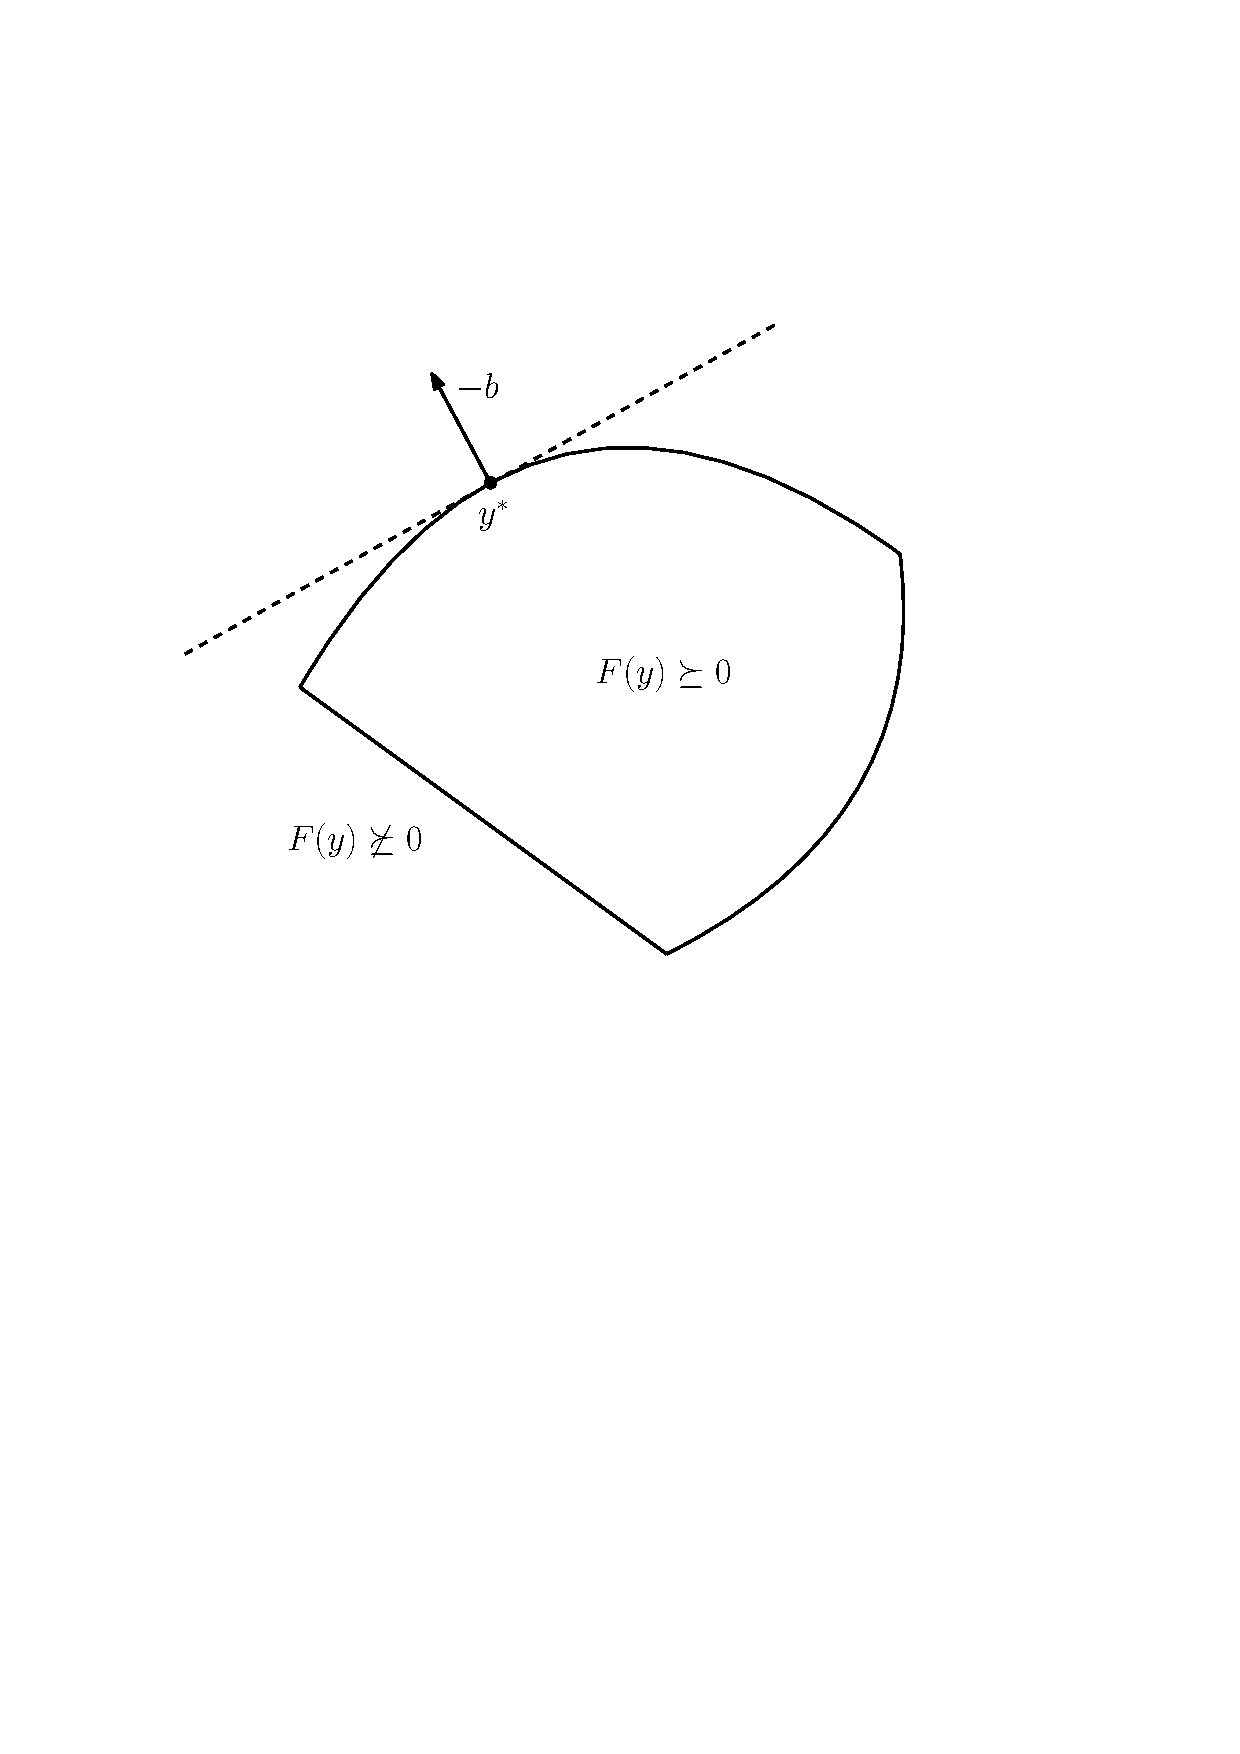
\includegraphics[width=0.5\textwidth]{drawings/SDP_problem.pdf}
  \caption{Example of a simple semidefinite problem for $y\in\R^2$. Boundary of the feasible set $\big\{y\ |\ F(y)\succeq 0\big\}$ is shown as a black curve. The minimal value of the objective function $b^\top y$ is attained at $y^*$.}
  \labelfig{SDP:prelim:problem}
\end{figure}

The optimal solution $y^*$ of any semidefinite program lies on the boundary of the feasible set, supposing the problem is feasible and the solution exists.
The boundary of the feasible set is not smooth in general, but it is piecewise smooth as each piece is an algebraic surface.

\begin{example}[Linear programming]
  Semidefinite programming can be seen as an extension to the linear programming since the componentwise inequalities between vectors in linear programming can be replaced by LMI.
  Consider a linear program in a standard form
  \begin{align}
    \arraycolsep=1.4pt
    \begin{array}{rclrcl@{\hskip0.5cm}l}
      y^* &=& \displaystyle \arg\min_{y\in\R^m} & \multicolumn{3}{l}{b^\top y} \\
      && \text{s.t.} & \displaystyle Ay - c &\geq& 0
    \end{array}
  \end{align}
  with $b\in\R^m$, $c\in\R^n$ and $A = \bmB a_1 & \cdots & a_m \bmE \in\R^{n\times m}$.
  This program can be transformed into the semidefinite program \refeqb{SDP:prelim:dual} by assigning
  \begin{align}
    C &= \diag(c),\\
    A_i &= \diag(a_i).
  \end{align}
\end{example}

\section{State of the art review}\labelsec{SDP:soa}
An early paper by R. Bellman and K. Fan about theoretical properties of semidefinite programs \cite{Bellman-Fan} was issued in 1963.
Later on, many researchers worked on the problem of minimizing the maximal eigenvalue of a symmetric matrix, which can be done by solving a semidefinite program.
Selecting a few from many: J. Cullum, W. Donath, P. Wolfe \cite{Cullum-Donath-Wolfe}, M. Overton \cite{Overton} and G. Pataki \cite{Pataki}.
In 1984, the interior-point methods for LPs solving were introduced by N. Karmarkar \cite{Karmarkar1984}.
It was the first reasonably efficient algorithm that solves LPs in polynomial time with excellent behavior in practise.
The interior-point algorithms were then extended to be able to solve convex quadratic programs.

In 1988, Y. Nesterov and A. Nemirovski \cite{Nesterov-Nemirovski} did an important breakthrough.
They showed that interior-point methods developed for LPs solving can be generalized to all convex optimization problems.
All that is required, is the knowledge of a self-concordant barrier function for the feasible set of the problem.
Y. Nesterov and A. Nemirovski have shown that a self-concordant barrier function exists for every convex set.
However, their proposed universal self-concordant barrier function and its first and second derivatives are not easily computable.
Fortunately for SDP, which is an important class of convex optimization programs, computable self-concordant barrier functions are known, and therefore the interior-point methods can be used.

Nowadays, there are many libraries and toolboxes that one can use for solving semidefinite programs.
They differ to each other in used methods and their implementations.
Before starting solving a problem, one should know the details of the problem to solve and choose the library accordingly to it as not every method and its implementation is suitable for the given problem.

Most methods are based on interior-point methods, which are efficient and robust for general semidefinite programs.
The main disadvantage of these methods is that they need to store and factorize usually large Hessian matrix.
Most modern implementations of the interior-point methods do not need the knowledge of an interior feasible point in advance.
SeDuMi \cite{sedumi} casts the standard semidefinite program into the homogeneous self-dual form, which has a trivial feasible point.
SDPA \cite{sdpa} uses an infeasible interior-point method, which can initialized by an infeasible point.
Some of the libraries (e.g.\ MOSEK \cite{mosek}) have started out as LPs solvers and were extended for QCQPs solving and convex optimization later on.

Another type of methods used in SDP are the first-order methods. 
They avoid storing and factorizing Hessian matrices, and therefore they are able to solve much larger problems than interior-point methods, but at some cost in accuracy.
This method is implemented, for instance, in the SCS solver \cite{scs}.

\section{Nesterov's approach}\labelsec{SDP:nesterov}
In this section, we will follow Chapter 4 of \cite{Nesterov-2004} by Y. Nesterov, which is devoted to the convex optimization problems.
This chapter describes the state of the art interior-point methods for solving convex optimization problems.
We will extract from it the only minimum, just to be able to introduce an algorithm for semidefinite programs solving.
We will present some basic definitions and theorems, but we will not prove them.
For the proofs and more details look into \cite{Nesterov-2004}.

\subsection{Self-concordant functions}
\begin{definition}[Self-concordant function in $\R$]
  A closed convex function $f: \R \mapsto \R$ is self-concordant if there exist a constant $M_f \geq 0$ such that the inequality
  \begin{align}
    |f'''(x)| &\leq M_f f''(x)^{3/2}
  \end{align}
  holds for all $x\in\dom f$.
\end{definition}

For better understanding of the self-concordant functions, we provide several examples.

\begin{example}~
  \begin{enumerate}
    \item Linear and convex quadratic functions.
      \begin{align}
        f'''(x) &= 0\ \text{ for all } x
      \end{align}
      Linear and convex quadratic functions are self-concordant with constant $M_f = 0$.
    \item Negative logarithms.
      \begin{align}
        f(x) &= -\ln(x)\ \text{ for } x>0\\
        f'(x) &= -\frac{1}{x}\\
        f''(x) &= \frac{1}{x^2}\\
        f'''(x) &= -\frac{2}{x^3}\\
        \frac{|f'''(x)|}{f''(x)^{3/2}} &= 2
      \end{align}
      Negative logarithms are self-concordant functions with constant $M_f = 2$.

    \item Exponential functions.
      \begin{align}
        f(x) &= e^x\\
        f''(x) \ =\ f'''(x) &= e^x\\
        \frac{|f'''(x)|}{f''(x)^{3/2}} &= e^{-x/2} \rightarrow+\infty \text{ as } x\rightarrow-\infty
      \end{align}
      Exponential functions are not self-concordant functions.
  \end{enumerate}
\end{example}

\begin{definition}[Self-concordant function in $\R^n$]
  A closed convex function $f: \R^n \mapsto \R$ is self-concordant if function $g: \R \mapsto \R$
  \begin{align}
    g(t) &= f(x + tv)
  \end{align}
  is self-concordant for all $x\in\dom f$ and all $v\in\R^n$.
\end{definition}

Now, let us focus on the main properties of the self-concordant functions.

\begin{theorem}
  Let functions $f_i$ be self-concordant with constants $M_i$  and let $\alpha_i > 0$, $i = 1,2$. Then the function
 \begin{align}
   f(x) &= \alpha_1f_1(x) + \alpha_2f_2(x)
 \end{align}
 is self-concordant with constant
 \begin{align}
   M_f &= \max \bigg\{\frac{1}{\sqrt{\alpha_1}}M_1;\ \frac{1}{\sqrt{\alpha_2}}M_2\bigg\}
 \end{align}
 and
 \begin{align}
   \dom f &= \dom f_1 \cap \dom f_2.
 \end{align}
\end{theorem}

\begin{corollary}\labelcol{SDP:scf:scaling}
  Let function $f$ be self-concordant with some constant $M_f$ and $\alpha > 0$. Then the function $\phi(x) = \alpha f(x)$ is also self-concordant with the constant $M_\phi = \frac{1}{\sqrt{\alpha}}M_f$.
\end{corollary}

We call function $f(x)$ as the standard self-concordant function if $f(x)$ is some self-concordant function with the constant $M_f = 2$. Using \refcol{SDP:scf:scaling}, we can see that any self-concordant function can be transformed into the standard self-concordant function by scaling.

\begin{theorem}\labelthe{SDP:scf:hessian}
  Let function $f$ be self-concordant. If $\dom f$ contains no straight line, then the Hessian $f''(x)$ is nondegenerate at any $x$ from $\dom f$.
\end{theorem}

For some self-concordant function $f(x)$, for which we assume, that $\dom f$ contains no straight line (which implies that all $f''(x)$ are nondegenerate, see \refthe{SDP:scf:hessian}), we denote two local norms as
\begin{align}
  \| u \|_x &= \sqrt{u^\top f''(x) u},\\
  \| u \|_x^* &= \sqrt{u^\top f''(x)^{-1} u}.
\end{align}

Consider minimization problem
\begin{align}
  x^* &= \arg\min_{x\in\dom f} f(x)\labeleq{SDP:scf:minProblem}
\end{align}
as the minimization of the self-concordant function $f(x)$.
\refalg{SDP:scf} describes the iterative process of solving the optimization problem \refeqb{SDP:scf:minProblem}.
The algorithm is divided into two stages by the value of $\|f'(x_k)\|_{x_k}^*$.
The splitting parameter $\beta$ guarantees quadratic convergence rate for the second part of the algorithm. The parameter $\beta$ is chosen from interval $(0, \bar{\lambda})$, where
\begin{align}
  \bar{\lambda} &= \frac{3 - \sqrt{5}}{2},
\end{align}
which is a root of the equation
\begin{align}
  \frac{\lambda}{(1-\lambda)^2} &= 1.
\end{align}

\begin{algorithm}[ht]
  \begin{algorithmic}[1]
    \Require
      \Statex $f$ a self-concordant function to minimize
      \Statex $x_0 \in \dom f$ a starting point
      \Statex $\beta \in (0,\bar{\lambda})$ a parameter of size of the region of quadratic convergence
      \Statex $\varepsilon$ a precision
    \Ensure
      \Statex $x^*$ an optimal solution to the minimization problem \refeqb{SDP:scf:minProblem}
      \Statex

    \State $k \gets 0$
    \While{$\|f'(x_k)\|_{x_k}^* \geq \beta$} \labelalgline{SDP:scf:w1b}
      \State $x_{k+1} \gets x_k - \frac{1}{1+\|f'(x_k)\|_{x_k}^*}f''(x_k)^{-1}f'(x_k)$
      \State $k \gets k + 1$
    \EndWhile \labelalgline{SDP:scf:w1e}
    \While{$\|f'(x_k)\|_{x_k}^* > \varepsilon$} \labelalgline{SDP:scf:w2b}
      \State $x_{k+1} \gets x_k - f''(x_k)^{-1}f'(x_k)$
      \State $k \gets k + 1$
    \EndWhile \labelalgline{SDP:scf:w2e}
    \State \Return $x^* \gets x_k$

  \end{algorithmic}
  \caption{Newton method for minimization of the self-concordant functions.}
  \labelalg{SDP:scf}
\end{algorithm}


The first while loop (lines \refalgline{SDP:scf:w1b} -- \refalgline{SDP:scf:w1e}) represents damped Newton method, where at each iteration we have
\begin{align}
  f(x_k) - f(x_{k+1}) &\geq \beta - \ln(1+\beta) \text{ for } k \geq 0,
\end{align}
where
\begin{align}
  \beta - \ln(1+\beta) &> 0 \text{ for } \beta > 0,
\end{align}
and therefore the global convergence of the algorithm is ensured.
It can be shown that the local convergence rate of the damped Newton method is also quadratic, but the presented switching strategy is preferred as it gives better complexity bounds.

The second while loop of the algorithm (lines \refalgline{SDP:scf:w2b} -- \refalgline{SDP:scf:w2e}) is the standard Newton method with quadratic convergence rate.

The algorithm terminates when the required precision $\varepsilon$ is reached.


\subsection{Self-concordant barriers}
To be able to introduce self-concordant barriers, let us denote $\Dom f = \cl(\dom f)$.

\begin{definition}[Self-concordant barrier]\labeldef{SDP:scb:scb}
  Let $F(x)$ be a standard self-concordant function. We call it a $\nu$-self-concordant barrier for set $\Dom F$, if
  \begin{align}
    \sup_{u\in\R^n} \big(2u^\top F'(x) - u^\top F''(x) u\big) &\leq \nu \labeleq{SDP:scb:def}
  \end{align}
  for all $x\in\dom F$. The value $\nu$ is called the parameter of the barrier.
\end{definition}

The inequality \refeqb{SDP:scb:def} can be rewritten into the following equivalent matrix notation:
\begin{align}
  F''(x) &\succeq \frac{1}{\nu}F'(x)F'(x)^\top.\labeleq{SDP:scb:def1}
\end{align}

In \refdef{SDP:scb:scb}, the hessian $F''(x)$ is not required to be nondegenerate. However, in case that $F''(x)$ is nondegenerate, the inequality \refeqb{SDP:scb:def} is equivalent to
\begin{align}
  F'^\top(x)F''(x)^{-1}F'(x) &\leq \nu.\labeleq{SDP:scb:def2}
\end{align}

Let us explore, which basic functions are self-concordant barriers.

\begin{example}~
  \begin{enumerate}
    \item Linear functions.
      \begin{align}
        F(x) &= \alpha + a^\top x,\ \dom F = \R^n\\
        F''(x) &= 0
      \end{align}
      From \refeqb{SDP:scb:def1} and for $a \neq 0$ follows, that linear functions are not self-concordant barriers.

    \item Convex quadratic functions.\\
      For $A = A^\top \succ 0$:
      \begin{align}
        F(x) &= \alpha + a^\top x + \frac{1}{2} x^\top Ax,\ \dom F = \R^n\\
        F'(x) &= a + Ax\\
        F''(x) &= A
      \end{align}
      After substitution into \refeqb{SDP:scb:def2} we obtain
      \begin{align}
        (a + Ax)^\top A^{-1}(a + Ax) &= a^\top A^{-1}a + 2a^\top x + x^\top Ax,
      \end{align}
      which is unbounded from above on $\R^n$. Therefore, quadratic functions are not self-concordant barriers.
      

    \item Logarithmic barrier for a ray.
      \begin{align}
        F(x) &= -\ln x,\ \dom F = \big\{x\in\R\ |\ x > 0\big\}\\
        F'(x) &= -\frac{1}{x}\\
        F''(x) &= \frac{1}{x^2}
      \end{align}
      From \refeqb{SDP:scb:def2}, when $F'(x)$ and $F''(x)$ are both scalars, we get
      \begin{align}
        \frac{F'(x)^2}{F''(x)} &= \frac{x^2}{x^2} = 1.
      \end{align}
      Therefore, the logarithmic barrier for a ray is a self-concordant barrier with parameter $\nu = 1$ on domain $\big\{x\in\R\ |\ x > 0\big\}$.
  \end{enumerate}
\end{example}

Now, let us focus on the main properties of the self-concordant barriers.

\begin{theorem}\labelthe{SDP:scb:penaltyFunction}
  Let $F(x)$ be a self-concordant barrier. Then the function $c^\top x + F(x)$ is a self-concordant function on $\dom F$.
\end{theorem}

\begin{theorem}
  Let $F_i$ be a $\nu_i$-self-concordant barriers, $i = 1,2$. Then the function
  \begin{align}
    F(x) &= F_1(x) + F_2(x)
  \end{align}
  is a self-concordant barrier for convex set
  \begin{align}
    \Dom F &= \Dom F_1 \cap \Dom F_2
  \end{align}
  with the parameter
  \begin{align}
    \nu &= \nu_1 + \nu_2.
  \end{align}
\end{theorem}

\begin{theorem}\labelthe{SDP:scb:distance}
  Let $F(x)$ be a $\nu$-self-concordant barrier. Then for any $x\in\Dom F$ and $y\in\Dom F$ such that
  \begin{align}
    (y-x)^\top F'(x) &\geq 0,
  \end{align}
  we have
  \begin{align}
    \|y-x\|_x &\leq \nu + 2\sqrt{\nu}.
  \end{align}
\end{theorem}

There is one special point of convex set, which is important for solving convex minimization problems.
It is called the analytic center of convex set and we will focus on its properties.

\begin{definition}
  Let $F(x)$ be a $\nu$-self-concordant barrier for the set $\Dom F$. The point
  \begin{align}
    x^*_F &= \arg \min_{x\in\Dom F} F(x) \labeleq{SDP:scb:ac}
  \end{align}
  is called the analytic center of convex set $\Dom F$, generated by the barrier $F(x)$.
\end{definition}

\begin{theorem}
  Assume that the analytic center of a $\nu$-self-concordant barrier $F(x)$ exists. Then for any $x\in\Dom F$ we have
  \begin{align}
    \|x-x^*_F\|_{x^*_F} &\leq \nu + 2\sqrt{\nu}.
  \end{align}
\end{theorem}

This property clearly follows from \refthe{SDP:scb:distance} and the fact that $F'(x^*_F) = 0$.

Thus, if $\Dom F$ contains no straight line, then the existence of $x^*_F$ (which leads to nondegenerate $F''(x^*_F)$) implies that the set $\Dom F$ is bounded.

Now, we describe the algorithm and its properties for obtaining an approximation to the analytic center.
To find the analytic center, we need to solve the minimization problem \refeqb{SDP:scb:ac}.
For that, we will use the standard implementation of the damped Newton method with a termination condition
\begin{align}
  \|F'(x_k)\|^*_{x_k} &\leq \beta \text{ for } \beta\in(0,1).
\end{align}
The pseudocode of the whole minimization process is shown in \refalg{SDP:scb:ac}.

\begin{algorithm}[ht]
  \begin{algorithmic}[1]
    \Require
      \Statex $F$ a self-concordant barrier
      \Statex $x_0 \in \Dom F$ a starting point
      \Statex $\beta \in (0,1)$ a centering parameter
    \Ensure
      \Statex $x^*_F$ an approximation of the analytic center of the set $\Dom F$
      \Statex

    \State $k \gets 0$
    \While{$\|F'(x_k)\|_{x_k}^* > \beta$}
      \State $x_{k+1} \gets x_k - \frac{1}{1+\|F'(x_k)\|_{x_k}^*}F''(x_k)^{-1}F'(x_k)$
      \State $k \gets k + 1$
    \EndWhile
    \State \Return $x^*_F \gets x_k$

  \end{algorithmic}
  \caption{Damped Newton method for analytic centers}
  \labelalg{SDP:scb:ac}
\end{algorithm}


\begin{theorem}
  \refalg{SDP:scb:ac} terminates no later than after $N$ steps, where
  \begin{align}
    N &= \frac{1}{\beta - \ln(1+\beta)}\big(F(x_0) - F(x^*_F)\big).
  \end{align}
\end{theorem}

The knowledge of the analytic center allows us to solve the standard minimization problem
\begin{align}
  x^* &= \arg\min_{x\in Q} c^\top x \labeleq{SDP:scb:standardProblem}
\end{align}
with bounded closed convex set $Q \equiv \Dom F$, which has nonempty interior, and which is endowed with a $\nu$-self-concordant barrier $F(x)$.
Denote
\begin{align}
  f(t,x) &= tc^\top x + F(x) \text{ for } t \geq 0
\end{align}
as a parametric penalty function.
Using \refthe{SDP:scb:penaltyFunction} we can see that $f(t,x)$ is self-concordant in $x$.
Let us introduce new minimization problem using the parametric penalty function $f(t,x)$
\begin{align}
  x^*(t) &= \arg\min_{x\in\dom F} f(t,x).\labeleq{SDP:scb:centralPath}
\end{align}
This trajectory is called the central path of the problem \refeqb{SDP:scb:standardProblem}.
We will reach the solution $x^*(t) \rightarrow x^*$ as $t \rightarrow +\infty$.
Moreover, since the set $Q$ is bounded, the analytic center $x^*_F$ of this set exists and
\begin{align}
  x^*(0) &= x^*_F.
\end{align}
From the first-order optimality condition, any point of the central path satisfies equation
\begin{align}
  tc + F'\big(x^*(t)\big) &= 0.
\end{align}
Since the analytic center lies on the central path and can be found by \refalg{SDP:scb:ac}, all we have to do, to find the solution $x^*$, is to follow the central path. 
This enables us an approximate centering condition:
\begin{align}
  \|f'(t,x)\|^*_x = \|tc + F'(x)\|^*_x &\leq \beta, \labeleq{SDP:scb:cntrCondition}
\end{align}
where the centering parameter $\beta$ is small enough.

Assuming $x\in\dom F$, one iteration of the path-following algorithm consists of two steps:
\begin{align}
  t_+ &= t + \frac{\gamma}{\|c\|^*_x},\\
  x_+ &= x - F''(x)^{-1}\big(t_+c+F'(x)\big).
\end{align}

\begin{theorem}
  Let $x$ satisfy the approximate centering condition \refeqb{SDP:scb:cntrCondition}
  \begin{align}
    \|tc + F'(x)\|^*_x &\leq \beta
  \end{align}
  with $\beta < \bar{\lambda} = \frac{3-\sqrt{5}}{2}$.
  Then for $\gamma$, such that
  \begin{align}
    |\gamma| &\leq \frac{\sqrt{\beta}}{1+\sqrt{\beta}} - \beta,
  \end{align}
  we have again
  \begin{align}
    \|t_+c + F'(x_+)\|^*_{x_+} &\leq \beta.
  \end{align}
\end{theorem}

This theorem ensures the correctness of the presented iteration of the path-following algorithm.
For the whole description of the path-following algorithm please see \refalg{SDP:scb:pf}.

\begin{algorithm}[ht]
  \begin{algorithmic}[1]
    \Require
      \Statex $F$ a $\nu$-self-concordant barrier
      \Statex $x_0 \in \dom F$ a starting point satisfying $\|F'(x_0)\|^*_{x_0} \leq \beta$, e.g.\ the analytic center $x^*_F$ of the set $\Dom F$
      \Statex $\beta \in (0,1)$ a centering parameter
      \Statex $\gamma$ a parameter satisfying $|\gamma| \leq \frac{\sqrt{\beta}}{1+\sqrt{\beta}} - \beta$
      \Statex $\varepsilon > 0$ an accuracy
    \Ensure
      \Statex $x^*$ an approximation to the optimal solution to the minimization problem \refeqb{SDP:scb:standardProblem}
      \Statex

    \State $t_0 \gets 0$
    \State $k \gets 0$
    \While{$\varepsilon t_k < \nu + \frac{(\beta + \sqrt{\nu})\beta}{1-\beta}$}
      \State $t_{k+1} \gets t_k + \frac{\gamma}{\|c\|^*_{x_k}}$
      \State $x_{k+1} \gets x_k - F''(x_k)^{-1}\big(t_{k+1}c + F'(x_k)\big)$
      \State $k \gets k + 1$
    \EndWhile
    \State \Return $x^* \gets x_k$

  \end{algorithmic}
  \caption{Path following algorithm. \cite[Scheme~4.2.23]{Nesterov-2004}}
  \labelalg{SDP:scb:pf}
\end{algorithm}


\begin{theorem}
  \refalg{SDP:scb:pf} terminates no more than after $N$ steps, where
  \begin{align}
    N &\leq \mathcal{O}\Bigg(\sqrt{\nu}\ln\frac{\nu \|c\|^*_{x^*_F}}{\varepsilon}\Bigg).
  \end{align}
\end{theorem}

The parameters $\beta$ and $\gamma$ in \refalg{SDP:scb:ac} and \refalg{SDP:scb:pf} can be fixed. The reasonable values are:
\begin{align}
  \beta &= \frac{1}{9},\labeleq{SDP:scb:beta}\\
  \gamma &= \frac{\sqrt{\beta}}{1+\sqrt{\beta}} - \beta = \frac{5}{36}.\labeleq{SDP:scb:gamma}
\end{align}

The union of \refalg{SDP:scb:ac} and \refalg{SDP:scb:pf} can be easily used to solve the standard minimization problem \refeqb{SDP:scb:standardProblem}, supposing we have a feasible point $x_0\in Q$.

\subsection{Barrier function for semidefinite programming}
In this section, we are going to show, how to find a self-concordant barrier for the semidefinite program \refeqb{SDP:prelim:dual}, so that we can use \refalg{SDP:scb:ac} and \refalg{SDP:scb:pf} to solve it.
For the purpose of this section, we are interested only in the constrains of the problem.
The constrains are defining us the feasibility set $Q$:
\begin{align}
  Q &= \bigg\{y\in\R^m\ |\ A_0 + \sum_{i=1}^mA_iy\ind i \succeq 0\bigg\},
\end{align}
where $A_0, \ldots, A_m \in\Sym^n$.
Let us denote $X(y) = A_0 + \sum_{i=1}^mA_iy\ind i$.
If the matrix $X(y)$ is block diagonal
\begin{align}
  X(y) &= \begin{bmatrix}
          X_1(y) & 0      & \cdots & 0      \\
          0      & X_2(y) & \cdots & 0      \\
          \vdots & \vdots & \ddots & \vdots \\
          0      & 0      & \cdots & X_k(y)
        \end{bmatrix} \labeleq{SDP:bf:bd}
\end{align}
with $X_j(y)\in\Sym^{n_j}$ for $j = 1, \ldots, k$ and $\sum_{j=1}^k n_j = n$, then the feasibility set $Q$ can be expressed as
\begin{align}
  Q &= \big\{y\in\R^m\ |\ X_j(y) \succeq 0,\ j = 1,\ldots, k\big\}.
\end{align}
This rule allows us to easily add or remove some constraints without touching the others and to keep the sizes of the used matrices small, which can significantly speed up the computation.

Instead of the set $Q$, which is parametrized by $y$, we can directly optimize over the set of positive semidefinite matrices. This set $\PSDCone^n$ is defined as
\begin{align}
  \PSDCone^n &= \big\{X\in\Sym^n\ |\ X\succeq0\big\}
\end{align}
and it is called the cone of positive semidefinite $n\times n$ matrices. This cone is a closed convex set, which interior is formed by positive definite matrices and on its boundary lie matrices, which have at least one eigenvalue equal to zero.

Now, we are looking for a self-concordant barrier function, which will enable us to optimize over the cone $\PSDCone^n$.
The domain of this function needs to contain the set $\PSDCone^n$ and the values of the function have to be growing to $+\infty$ as getting closer to the boundary of the set $\PSDCone^n$.
This will create us a repelling force from the boundary of $\PSDCone^n$, when following the central path \refeqb{SDP:scb:centralPath}.
Consider the function $F(X)$ as the self-concordant barrier function for the set $\PSDCone^n$:
\begin{align}
  F(X) &= -\ln\prod_{i=1}^{n}\lambda_i(X),
\end{align}
where $X\in\inter\PSDCone^n$ and $\big\{\lambda_i(X)\big\}_{i=1}^n$ is the set of eigenvalues of the matrix $X$.
To avoid the computation of eigenvalues, the function $F(X)$ can be also expressed as:
\begin{align}
  F(X) &= -\ln\det(X).
\end{align}

\begin{theorem}\labelthe{SDP:bf:nu}
  Function $F(X)$ is an $n$-self-concordant barrier for $\PSDCone^n$.
\end{theorem}

\begin{example}
  Consider one-dimensional problem with linear constraint $x \geq 0$.
  Then, the set $Q$ is
  \begin{align}
    Q &= \{x\in\R\ |\ x \geq 0\}
  \end{align}
  and one of the barrier functions for this set $Q$ is
  \begin{align}
    F(x) &= -\ln(x).
  \end{align}
  Then, when following the central path \refeqb{SDP:scb:centralPath}, the function $F(x)$ allows us to reach the boundary of $Q$ as $t$ grows to $+\infty$.
  This situation is showed in \reffig{SDP:bf:barrier} for different values of $t$.

  \begin{figure}[ht]
    \centering
    \resizebox{0.95\textwidth}{!}{\input{graphs/SDP_barrier}}
    \caption{Illustration of the logarithmic barrier function for different values of $t$.}
    \labelfig{SDP:bf:barrier}
  \end{figure}
\end{example}

Note, that $\Dom F \supseteq \PSDCone^n$ because $\det(X) \geq 0$ when the number of negative eigenvalues of $X$ is even. Therefore, the set $\Dom F$ is made by disjoint subsets, which one of them is $\PSDCone^n$. As \refalg{SDP:scb:ac} and \refalg{SDP:scb:pf} are interior point algorithms, when the starting point is from $\inter\PSDCone^n$, then we never leave $\PSDCone^n$ during the execution of the algorithms and the optimal solution is found.

Similarly, the self-concordant barrier function for the set $Q$ is a function 
\begin{align}
  F(y) &= -\ln\det\!\big(X(y)\big). \labeleq{SDP:bf:bfy}
\end{align}

\begin{example}
  To make it clearer, what is the difference between the set $Q$ and $\Dom F(y)$, we have prepared this example. Let
  \begin{align}
    X(y) &= \bmB y_2 & y_1 \\ y_1 & y_2 \bmE,
  \end{align}
  where $y = \bmB y_1 & y_2 \bmE^\top$. The equation
  \begin{align}
    z &= \det\!\big(X(y)\big) = y_2^2 - y_1^2
  \end{align}
  represents a hyperbolic paraboloid, which you can see in \reffig{SDP:bf:hyperPar}.
  Therefore, the equation $z = 0$ is a slice of it, denoted by the purple color in \reffig{SDP:bf:hyperParSlice}. The domain of the self-concordant barrier function is
  \begin{align}
    \Dom F(y) &= \Big\{y\ |\ \det\!\big(X(y)\big) \geq 0\Big\}\labeleq{SDP:bf:domF}
  \end{align}
  and is shaded by the blue color.
  We can see, that the set $\Dom F(y)$ consists of two disjoint parts. One of them is the set, where $X(y)\succeq0$ (denoted by the orange color) and the second part is an area, where both eigenvalues of $X(y)$ are negative.
  Therefore, one has to pick his starting point $x_0$ from the interior of the set $Q = \big\{y\in\R^2\ |\ X(y) \succeq 0\big\}$ to obtain the optimal solution from the set $Q$.

  \begin{figure}[ht]
    \centering
    \resizebox{0.95\textwidth}{!}{\input{graphs/SDP_hyperPar}}
    \caption{Hyperbolic paraboloid $z = y_2^2 - y_1^2$.}
    \labelfig{SDP:bf:hyperPar}
  \end{figure}

  \begin{figure}[ht]
    \centering
    \resizebox{0.95\textwidth}{!}{\input{graphs/SDP_hyperParSlice}}
    \caption{Illustration of the sets $\Dom F(y)$ and $\big\{y\ |\ X(y) \succeq 0\big\}$.}
    \labelfig{SDP:bf:hyperParSlice}
  \end{figure}
\end{example}

When the matrix $X$ has the block diagonal form \refeqb{SDP:bf:bd}, we can rewrite the barrier function \refeqb{SDP:bf:bfy} into summation form
\begin{align}
  F(y) &= -\sum_{j=1}^k \ln\det\!\big(X_j(y)\big).
\end{align}
For the purposes of \refalg{SDP:scb:ac} and \refalg{SDP:scb:pf}, we need the first and the second partial derivatives of this function.
Let us denote $X_j(y) = A_{j, 0} + \sum_{i=1}^mA_{j, i}y\ind i$ for $j = 1, \ldots, k$, then the derivatives are:
\begin{align}
  \frac{\partial F}{\partial y\ind u}\big(y\big) &= -\sum_{j=1}^k \tr\!\big(X_j(y)^{-1}A_{j,u}\big),\\
  \frac{\partial^2 F}{\partial y\ind u \partial y\ind v}\big(y\big) &= \sum_{j=1}^k \tr\!\Big(\!\big(X_j(y)^{-1}A_{j,u}\big)\big(X_j(y)^{-1}A_{j,v}\big)\!\Big),
\end{align}
for $u, v = 1,\ldots, m$.

The computation of the derivatives is the most expensive part of each step of \refalg{SDP:scb:ac} and \refalg{SDP:scb:pf}.
Therefore, the estimated number of arithmetic operations of computation of the derivatives is also the complexity of each step in the algorithms.
The number of arithmetic operations for $j$-th constraint in form $\big\{y\ |\ X_j(y) \succeq 0\big\}$ is:
\begin{itemize}
  \item the computation of $X_j(y) = A_{j,0} + \sum_{i=1}^mA_{j,i}y\ind i$ needs $mn^2$ operations,
  \item the computation of the inversion $X_j(y)^{-1}$ needs $n^3$ operations,
  \item to compute all matrices $X_j(y)^{-1}A_{j,u}$ for $u = 1,\ldots,m$ is needed $mn^3$ operations,
  \item to compute $\tr\!\big(X_j(y)^{-1}A_{j,u}\big)$ for $u = 1,\ldots,m$ is needed $mn$ operations,
  \item the computation of $\tr\!\Big(\!\big(X_j(y)^{-1}A_{j,u}\big)\big(X_j(y)^{-1}A_{j,v}\big)\!\Big)$ for $u, v = 1,\ldots, m$ needs $m^2n^2$ operations.
\end{itemize}
The most expensive parts requires $mn^3$ and $m^2n^2$ arithmetic operations on each constraint.
Typically, the value $k$, the number of constraints, is small and it keeps constant, when the semidefinite programs are generated as subproblems, when solving more complex problems, e.g.\ polynomial optimization. Therefore, we can say, that $k$ is constant and we can omit it from the complexity estimation.
To sum up, one step of \refalg{SDP:scb:ac} and \refalg{SDP:scb:pf} requires
\begin{align}
  \mathcal{O}\big(m(m+n)n^2\big)\labeleq{SDP:bf:O}
\end{align}
arithmetic operations.

\section{Implementation details}\labelsec{SDP:impl}
To be able to study the algorithms described previously in this section, we have implemented them in the programming language Python \cite{python}.
The full knowledge of the code allows us to trace the algorithms step by step and inspect their behaviors.
Instead of using some state of the art toolboxes for semidefinite programming, e.g.\ SeDuMi \cite{sedumi} and MOSEK \cite{mosek}, which are more or less black boxes for us, the knowledge of the used algorithms allows us to decide, if the chosen algorithm is suitable for the given semidefinite problem or not.
Moreover, if we would like to create some specialized solver for some class of semidefinite problems, we can easily reuse the code, edit it as required and build the solver very quickly.
On the other hand, we can not expect that our implementation will be as fast as the implementation of some state of the art toolboxes, as much more time and people was used to develop them.

The implementation is compatible with Python version 3.5 and higher.
The package NumPy is used for linear algebra computations.
Please refer to the installation guide of NumPy for your system to ensure, that it is correctly set to use the linear algebra libraries, e.g.\ LAPACK \cite{lapack}, ATLAS \cite{atlas} and BLAS \cite{blas}.
The incorrect setting of these libraries causes significant drop of the performance.
Other Python packages are required as well, e.g.\ SymPy and SciPy, but theirs settings are not so crucial for the performance of this implementation.

\subsection{Package installation}\labelsec{SDP:install}
The package with implementation of \refalg{SDP:scb:ac} and \refalg{SDP:scb:pf} is named Polyopt, as the semidefinite programming part of this package is only a tool, which is  used for polynomial optimization and polynomial systems solving, which will be described in \refcha{POP}.
The newest version of the package is available at \url{http://cmp.felk.cvut.cz/~trutmpav/master-thesis/polyopt/}.
To install the package on your system, you have to clone and checkout the Git repository with the source codes of the package.
To install other packages that are required, the preferred way is to use the pip\footnote{The PyPA recommended tool for installing Python packages. See \url{https://pip.pypa.io}.} installer. The required packages are listed in the \texttt{requirements.txt} file.
Then, install the package using the script \texttt{setup.py}.
For the exact commands for the whole installation process please see \reflis{SDP:imp:install}.
\begin{lstlisting}[language=bash, caption={Installation of the package Polyopt.}, labellis={SDP:imp:install}]
git clone https://github.com/PavelTrutman/polyopt.git
cd polyopt
pip3 install -r requirements.txt
python3 setup.py install
\end{lstlisting}
To check, whether the installation was successful, run command \texttt{python3 setup.py test}, which will execute the predefined tests.
If no error emerges, then the package is installed and ready to use.

\subsection{Usage}
The Polyopt package is created to be able to solve semidefinite programs in a form
\begin{align}
  \arraycolsep=1.4pt
  \begin{array}{rclrcl@{\hskip0.5cm}l}
    y^* &=& \displaystyle \arg\min_{y\in\R^m} & \multicolumn{3}{l}{c^\top y} \\
    && \text{s.t.} & \displaystyle A_{j,0} + \sum_{i=1}^m A_{j,i}y\ind i &\succeq& 0 & \text{ for } j = 1,\ldots,k,
  \end{array}\labeleq{SDP:imp:problem}
\end{align}
where $A_{j,i}\in\Sym^{n_j}$ for $i = 0,\dots m$ and $j=1,\dots,k$, $c\in\R^m$ and $k$ is the number of constraints.
In addition, a strictly feasible point $y_0\in\R^m$ must be given.

The semidefinite program solver is implemented in the class \texttt{SDPSolver} of the Polyopt package. Firstly, the problem is initialized by the matrices $A_{j,i}$ and the vector $c$.
Then, the function \texttt{solve} is called with parameter $y_0$ as the starting point and with the method for the analytic center estimation.
A choice from two methods is available, firstly, the method \texttt{dampedNewton}, which corresponds to \refalg{SDP:scb:ac}, and secondly, the method \texttt{auxFollow}, which is the implementation of the Auxiliary path-following scheme \cite{Nesterov-2004}. 
However, the \texttt{auxFollow} method is unstable and it fails in some cases, and therefore it is not recommended to use.
The function \texttt{solve} returns the optimal solution $y^*$.
The minimal working example is shown in \reflis{SDP:imp:usage}.
\begin{lstlisting}[language=python, caption={Typical usage of the class \texttt{SDPSolver} of the Polyopt package.}, labellis={SDP:imp:usage}]
import polyopt

# supposing the matrices Aij and the vectors c and y0 are already defined
problem = polyopt.SDPSolver(c, [[A10, A11, ..., A1m], ..., [Ak0, Ak1, ..., Akm]])
yStar = problem.solve(y0, problem.dampedNewton)
\end{lstlisting}

Detailed information can be printed out during the execution of the algorithm.
This option can be set by \texttt{problem.setPrintOutput(True)}.
Then, in each iteration of \refalg{SDP:scb:ac} and \refalg{SDP:scb:pf}, the values $k$, $x_k$ and eigenvalues of $X_j(x_k)$ are printed to the terminal.

If $n$, the dimension of the problem, is equal to 2, boundary of the set $\Dom F$ \refeqb{SDP:bf:domF} and all intermediate points $x_k$ can be plotted.
This can be enabled by setting \texttt{problem.setDrawPlot(True)}.
An example of such a graph is shown in \reffig{SDP:imp:demo}.

The parameters $\beta$ and $\gamma$ are predefined to the same values as in \refeqb{SDP:scb:beta} and \refeqb{SDP:scb:gamma}.
These parameters can be set to different values by assigning to the variables \texttt{problem.beta} and \texttt{problem.gamma} respectively.
The default value for the accuracy parameter $\varepsilon$ is $10^{-3}$.
This value can be changed by overwriting the variable \texttt{problem.eps}.

The function \texttt{problem.getNu()} returns the $\nu$ parameter of the self-concordant barrier function used for the problem according to \refthe{SDP:bf:nu}.
When the problem is solved, we can obtain the eigenvalues of $X(y^*)$ by calling \texttt{problem.eigenvalues()}.
We should observe, that some of them are positive and some of them are zero (up to the numerical precision).
The zero eigenvalues mean, that we have reached the boundary of the set $Q$, because the optimal solution lies always on the boundary of the set $Q$.

It may happen, that the set $\Dom F$ is not bounded, but the optimal solution can be attained.
In this case, the analytic center does not exists and the proposed algorithms can not be used. 
By adding a constraint 
\begin{align}
  X_{k+1}(y) &= \bmB R^2 & y\ind1 & y\ind2 & \cdots & y\ind m\\
                      y\ind1 & 1 & 0 & \cdots & 0\\
                      y\ind2 & 0 & 1 & \cdots & 0\\
                      \vdots & \vdots & \vdots & \ddots & \vdots\\
                      y\ind m & 0 & 0 & \cdots & 1\bmE \text{ for } R\in\R, \labeleq{SDP:imp:bound}
\end{align}
we bound the set by a ball with radius $R$.
The constraint \refeqb{SDP:imp:bound} is equivalent to
\begin{align}
  \|y\|_2^2 &\leq R^2.
\end{align}
This will make the set $\Dom F$ bounded and the analytic center can by found in the standard way by \refalg{SDP:scb:ac}.
When optimizing the linear function by \refalg{SDP:scb:pf}, the radius $R$ may be set too small and the optimum may be found on the boundary of the constraint \refeqb{SDP:imp:bound}.
Then, the found optimum is not the solution to the original problem and the algorithm has to be run again with bigger value of $R$.
The optimum is found on the boundary of the constraint \refeqb{SDP:imp:bound}, if at least one of the eigenvalues of $X_{k+1}(y^*)$ is zero.
In our implementation, the artificial bounding constraint \refeqb{SDP:imp:bound} can be set by \texttt{problem.bound(R)}.
When the problem is solved, we can list the eigenvalues of $X_{k+1}(y^*)$ by the function \texttt{problem.eigenvalues('bounded')}.

\begin{example}\labelex{SDP:imp:demo}
  Let us present a simple example to show a detailed usage of the package Polyopt.
  Let us have semidefinite program in a form
  \begin{align}
    \arraycolsep=1.4pt
    \begin{array}{rclrcl@{\hskip0.5cm}l}
      y^* &=& \displaystyle \arg\min_{y\in\R^2} & \multicolumn{3}{l}{y\ind1 + y\ind2} \\
      && \text{s.t.} & \displaystyle \bmB 1 +y\ind1 & y\ind2 & 0\\ y\ind2 & 1 -y\ind1& y\ind2\\ 0 & y\ind2 & 1-y\ind1 \bmE &\succeq& 0
    \end{array}
  \end{align}
  with starting point
  \begin{align}
    y_0 &= \bmB 0 & 0\bmE^\top.
  \end{align}
  \reflis{SDP:imp:demo} shows the Python code used to solve the given problem.
  The graph of the problem is showed in \reffig{SDP:imp:demo}.
  The analytic center of the feasible region of the problem is
  \begin{align}
    y_F^* &= \bmB -0.317 & 0\bmE^\top,
  \end{align}
  the optimal solution is attained at
  \begin{align}
    y^* &= \bmB -0.778 & -0.592 \bmE^\top
  \end{align}
  and the objective function has value $-1.37$.
  The eigenvalues of $X(y^*)$ are
  \begin{align}
    \Big\{\lambda_i\big(X(y^*)\big)\Big\}_{i=1}^3 &= \{2.32\cdot10^{-4};\ 1.32;\ 2.45\}.
  \end{align}

  \begin{lstlisting}[float, language=python, caption={Code for solving semidefinite problem stated in \refex{SDP:imp:demo}.}, labellis={SDP:imp:demo}]
from numpy import *
import polyopt

# Problem statement
# min c1*y1 + c2*y2
# s.t. A0 + A1*y1 + A2*y2 >= 0
c = array([[1], [1]])
A0 = array([[1,  0,  0],
            [0,  1,  0],
            [0,  0,  1]])
A1 = array([[1,  0,  0],
            [0, -1,  0],
            [0,  0, -1]])
A2 = array([[0,  1,  0],
            [1,  0,  1],
            [0,  1,  0]])

# starting point 
y0 = array([[0], [0]])

# create the solver object
problem = polyopt.SDPSolver(c, [[A0, A1, A2]])

# enable graphs
problem.setDrawPlot(True)

# enable informative output
problem.setPrintOutput(True)

# solve!
yStar = problem.solve(y0, problem.dampedNewton)

# print eigenvalues of X(yStar)
print(problem.eigenvalues())
  \end{lstlisting}

  \begin{figure}[ht]
    \centering
    \resizebox{0.95\textwidth}{!}{\input{graphs/SDP_demo}}
    \caption{Graph of the semidefinite optimization problem stated in \refex{SDP:imp:demo}.}
    \labelfig{SDP:imp:demo}
  \end{figure}
\end{example}

\section{Comparison with the state of the art methods}\labelsec{SDP:comparision}
\input{macros/SDP_performance}
Because a new implementation of a well-known algorithm was made, one should compare many properties of this implementation with the contemporary state of the art methods.
For that reason, we have generated some random instances of semidefinite problems.
We have solved these problems by our implementation from the Polyopt package and by selected state of the art toolboxes, namely SeDuMi \cite{sedumi} and MOSEK \cite{mosek}.
Firstly, we have verified the correctness of the implementation by checking that the optimal solution is the same as the solution obtained by SeDuMi and MOSEK for each instance of data.
We have also measured execution times of all three libraries and compared them in \reftab{SDP:perf:times} and \reffig{SDP:perf:times}.

\subsection{Problem description}
Now, let us describe, how the random instances of the semidefinite problems were generated.
From \refeqb{SDP:bf:O} we know that each step of \refalg{SDP:scb:ac} and \refalg{SDP:scb:pf} requires $m(m+n)n^2$ arithmetic operations, where $m$ is the size of the matrices in the LMI constraint and $n$ is the number of variables.
Since in typical applications of SDP, the size of the matrices grows with the number of variables, we have set $m = n$ to have just single parameter, which we call the size of the problem.

In our experiment, we have generated \importSDPPerformanceUnique{} unique LMI constraints for each size of the problem from \importSDPPerformanceDimMin{} to \importSDPPerformanceDimMax{}.
Each unique constraint has form
\begin{align}
  X_{k,l}(y) &= \Iden k + \sum_{i=1}^k A_{k,l,i} y\ind i\labeleq{SDP:perf:constr}
\end{align}
for the size of the problem $k = \importSDPPerformanceDimMin, \ldots, \importSDPPerformanceDimMax$ and unique LMI constraint $l = 1,\ldots, \importSDPPerformanceUnique$, where $A_{k,l,i}\in\Sym^k$.
The matrices $A_{k,l,i}$ were filled with random numbers from uniform distribution $(-1;1)$ with symmetricity of the matrices preserved.
The package Polyopt requires the starting point $y_0$ to be given by the user in advance.
But from the structure of the constraint \refeqb{SDP:perf:constr} we can see that $y_0\in\R^k$
\begin{align}
  y_0 &= \bmB 0 & \cdots & 0\bmE^\top
\end{align}
is a feasible point.
We used the point $y_0$ to initialize problems for Polyopt package, but we have let SeDuMi and MOSEK use their own initialization process. 
However, since the LMI constraints were randomly generated, there is no guarantee that the sets, which they define, are bounded.
Therefore, we have added constraint \refeqb{SDP:imp:bound} for $R = \importSDPPerformanceBound$, which guarantees that we are optimizing over bounded sets.

The objective function of the problem is generated randomly too.
For each unique instance, we have generated random vector $r\in\R^n$ from uniform distribution $(-1;1)$.
Then, the objective function to minimize is $r^\top y$.
The final generated problem denoted as $P_{k,l}$ looks like
\begin{align}
  \arraycolsep=1.4pt
  \begin{array}{rclrcl@{\hskip0.5cm}l}
    && \displaystyle \min_{y\in\R^k} & \multicolumn{3}{l}{r_{k,l}^\top y} \\
    && \text{s.t.} & \displaystyle \Iden k + \sum_{i=1}^k A_{k,l,i} y\ind i &\succeq& 0 \\
    &&& \bmB R^2 & y\ind1 & y\ind2 & \cdots & y\ind k\\
          y\ind1 & 1 & 0 & \cdots & 0\\
          y\ind2 & 0 & 1 & \cdots & 0\\
          \vdots & \vdots & \vdots & \ddots & \vdots\\
          y\ind k & 0 & 0 & \cdots & 1\bmE &\succeq& 0.
 \end{array}
\end{align}

\subsection{Time measuring}
To eliminate influences that negatively affect the execution times on CPU, such as other processes competing for the same CPU core, processor caching, data loading delays, etc., we have executed each problem $P_{k,l}$ \importSDPPerformanceRepeat{} times.
So, for each problem $P_{k,l}$ we have obtained execution times $\tau_{k,l,s}$ for $s = 1,\ldots,\importSDPPerformanceRepeat$.
Because the influences mentioned above can only prolong the execution times, we have selected minimum of $\tau_{k,l,s}$ for each problem $P_{k,l}$.
\begin{align}
  \tau_{k,l} &= \min_{s=1}^{\importSDPPerformanceRepeat} \tau_{k,l,s}
\end{align}
Since the execution times of problems of the same sizes should be more or less the same, we have computed the average execution time $\tau_k$ for each size of the problem.
\begin{align}
  \tau_k &= \frac{1}{\importSDPPerformanceUnique}\sum_{l=1}^{\importSDPPerformanceUnique} \tau_{k,l}
\end{align}
These execution times $\tau_k$, where $k$ is the size of the problem, were measured and computed separately for the Polyopt, SeDuMi and MOSEK toolboxes and are shown in \reftab{SDP:perf:times} and \reffig{SDP:perf:times}.

\begin{table}[ht]
  \centering
  \input{tables/SDP_performance.tex}
  \caption{Execution times of different sizes of semidefinite problems solved by the selected toolboxes.}
  \labeltab{SDP:perf:times}
\end{table}

\begin{figure}[ht]
  \centering
  \resizebox{0.95\textwidth}{!}{\input{graphs/SDP_performance}}
  \caption{Graph of execution times based on the size of semidefinite problems solved by the selected toolboxes.}
  \labelfig{SDP:perf:times}
\end{figure}

It has to be mentioned, that the Polyopt toolbox is implemented in Python, but the toolboxes SeDuMi and MOSEK were run from MATLAB with precompiled MEX files (compiled C, \CC{} or Fortran code) and therefore the execution times are not readily comparable.
On the other side, the Python package NumPy uses common linear algebra libraries, like LAPACK \cite{lapack}, ATLAS \cite{atlas} and BLAS \cite{blas}, and we can presume that SeDuMi and MOSEK use them too.

Our intention was to measure only the execution time of the solving phase, not of the preparation time.
In case of the Polyopt package, we measured the execution time of the function \texttt{solve()}.
For SeDuMi and MOSEK, we have used MATLAB framework YALMIP \cite{yalmip} for defining the semidefinite programs and calling the solvers.
The execution time of the YALMIP code is quite long, because YALMIP makes an analysis of the problem and compiles it into a standard form.
Only after that, an external solver (SeDuMi or MOSEK) is called to solve the problem.
Fortunately, YALMIP internally measures the execution time of the solver, so we have used this time in our statistics.

The experiments were executed on Intel Core i5-3210M CPU 2.50 GHz based computer with sufficient amount of free system memory.
The installed version of Python was 3.5.3 and MATLAB R2016b 64-bit was used.

\subsection{Results}
By the look of the graph in \reffig{SDP:perf:times}, we can see that the MOSEK toolbox totally wins.
The SeDuMi toolbox seems to have some constant overhead, but the execution time grows slowly with the increasing size of the problem.
The Polyopt package accomplishes quite bad results compared to SeDuMi and MOSEK, especially for large sizes of problems.
But this behavior was expected, as we know that the execution time should be proportional to $k^4$, where $k$ is the size of the problem.
However, due to SeDuMi overhead, the Polyopt package is faster than SeDuMi for problem sizes up to 8.

\section{Speed--accuracy trade-off}

\input{macros/SDP_prec_eps}
\begin{figure}[ht]
  \centering
  \resizebox{0.95\textwidth}{!}{\input{graphs/SDP_prec_eps_times}}
  \caption{TODO: Graph of execution times based on the size of semidefinite problems solved by the selected toolboxes.}
  \labelfig{TODO:SDP:perf:times}
\end{figure}

\begin{figure}[ht]
  \centering
  \resizebox{0.95\textwidth}{!}{\input{graphs/SDP_prec_eps_iters}}
  \caption{TODO: Graph of execution times based on the size of semidefinite problems solved by the selected toolboxes.}
  \labelfig{TODO:SDP:perf:times}
\end{figure}

\input{macros/SDP_prec_perc}
\begin{figure}[ht]
  \centering
  \resizebox{0.95\textwidth}{!}{\input{graphs/SDP_prec_perc_iters}}
  \caption{TODO: Graph of execution times based on the size of semidefinite problems solved by the selected toolboxes.}
  \labelfig{TODO:SDP:perf:times}
\end{figure}
